\documentclass[a4paper,10pt]{scrartcl}
\usepackage[top=2.5cm, bottom=2cm, left=2.5cm, right=2.5cm]{geometry}

% UTF-8 support
\usepackage[utf8]{inputenc}

% german and english language support
\usepackage[english,ngerman]{babel}

% more math symbols
\usepackage{amsmath}

% advanced tables
\usepackage{tabularx}

% hide the hyperlinks
\usepackage[hidelinks]{hyperref}

% no newpage after include
\usepackage{newclude}

% fancy graphics
\usepackage{graphicx}

% more customizable captions
\usepackage{caption}

% nice font
\usepackage{lmodern}

% ???
\usepackage{textcomp}
% \usepackage[onehalfspacing]{setspace}
\linespread{1}

% Tikz for designing graphics
\usepackage{tikz}
\usetikzlibrary{positioning}

% code
\usepackage{listings}
\lstset{ %
  frame=single,	                   % adds a frame around the code
  language=Python,                 % the language of the code
  % numbers=left,                    % where to put the line-numbers; possible values are (none, left, right)
  % stepnumber=1,                    % the step between two line-numbers. If it's 1, each line will be numbered
}

% hyperref / hyperlink settings
\usepackage{hyperref}
\hypersetup{
colorlinks,
citecolor=black,
filecolor=black,
linkcolor=black,
urlcolor=black
}

% renew some commands
\newcommand{\bold}{\textbf}
\renewcommand{\arraystretch}{1.5}
\newcommand{ \rarrow }{\( \rightarrow \)}

% redefine some parameters
\setlength\parindent{0pt}
\setlength\parskip{10pt}
\setlength{\footskip}{30pt}
\setcounter{tocdepth}{3}

%%% MAIN DOCUMENT BEGINS HERE %%%

\begin{document}

% titlepage settings
\title{Galaxy Generation}
\subtitle{Jugend Forscht \the\year}
\author{ Emile Hansmaennel \texttt{ emile.hansmaennel@gmail.com }}
\date{\today}

% generate the title using the informations given above
\maketitle

% include a nice image
\begin{figure}[h]
  \centering
  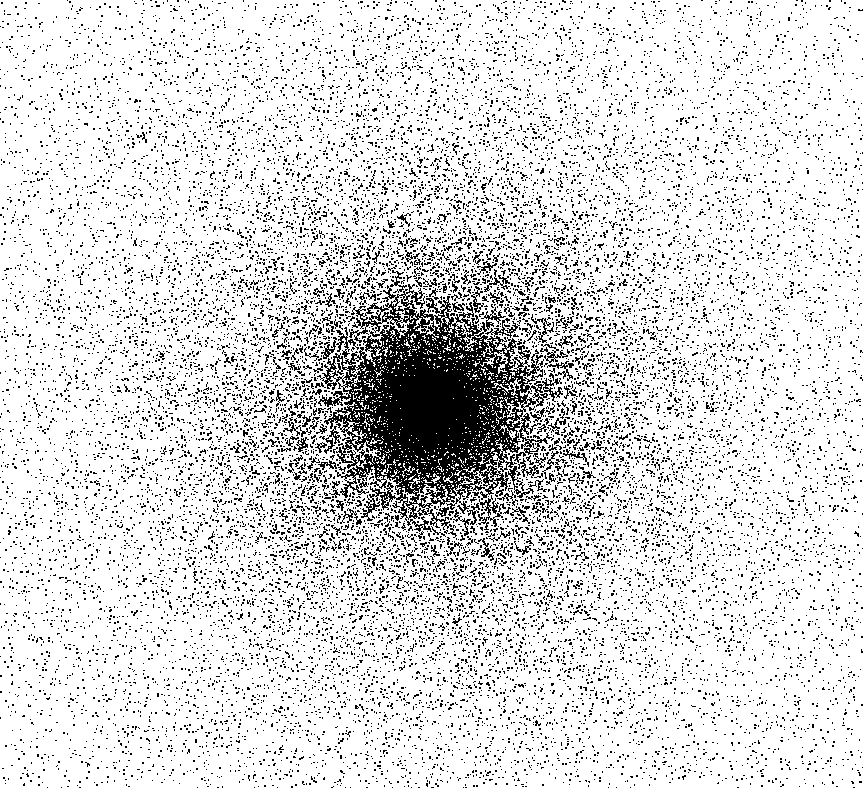
\includegraphics[width=120mm, trim={0 8.5cm 0 8.5cm}, clip]{figs/galaxy}
  \captionsetup{labelformat=empty}
  \caption{}
 \end{figure}

% include the abstract
\begin{abstract}
\include*{docs/1_kurzfassung}
\end{abstract}

% don't insert a page number on the first page
\thispagestyle{empty}
\clearpage
\newpage
\setcounter{page}{1}

% generate a table of contents
\tableofcontents
\newpage

\section{Einleitung} \label{Einleitung}
\include*{docs/2_einleitung}
\newpage

\section{Hauptteil} \label{Hauptteil}
\include*{docs/3_hauptteil}
\newpage

\section{Ergebnisse} \label{ergebnisse}
\include*{docs/4_ergebnisse}
\newpage

\section{Quellen und Hilfen} \label{quellen}
\include*{docs/5_quellen}
\newpage

\section{Nach der Abgabe...} \label{nach_der_abgabe}
\include*{docs/6_abgabe}

\end{document}
